

\begin{otherlanguage}{finnish}
\chapter*{Tekoälyavusteinen käyttäjän\\manipulointi\label{chapter:finnish}}
\begin{comment}
- erikoismerkkeinä piiloutuva tavutusohje ja sanarajaa luomaton välilyönti
- pitää olla viimeisteltyä kirjakieltä (ei alan slangia: koneiden kaatumisia...)
- taitto on siisti
- marginaaliin valuvat pitkät sanat katkaistaan
- (ali)luvun viimeiset ja ensimmäiset rivit pakotetaan samalle sivulle yhteenkuuluvien kanssa (tai tuomaan mukanaan toinenkin rivi)

\end{comment}


Moderni tekoäly on tuonut mukanaan uusia haasteita käyttäjän manipulointihyökkäyksiltä puolustautumiseen. Tässä lyhennelmässä esitellään tärkeimmät tekoälyavustetut organisaatioihin kohdistuvat käyttäjän manipulointihyökkäykset sekä puolustuskeinoja niihin. \textbf{Käyttäjän manipuloinnilla} (\textit{social engineering}) tarkoitetaan tietoturvan yhteydessä loppukäyttäjään eli ihmiseen kohdistuvaa tietoturvahyökkäystä~\citep{hatfield_SE_Evolution_Concept_2018}. Sen sijaan, että hyökkääjät etsisivät tietojärjestelmistä teknisiä haavoittuvuuksia, he kohdistavatkin hyökkäykset käyttäjään hyödyntäen psykologisia menetelmiä~\citep{wang_Defining_Social_Engineering_2020}.

Historiallisesti käyttäjän manipulointi on ollut riippuvainen ihmisen intuitiosta ja manuaalisesta työstä, mutta nyt moderni \textbf{tekoäly} (\textit{artificial intelligence, AI}) on muuttamassa kenttää~\citep{blauth_AI_Crime_Overview_Malicious_Use_Abuse_2022, king_AI_Crime_Interdisciplinary_Analysis_2019, mirsky_Threat_Offensive_AI_Organizations_2023}. Tekoälyn avulla hyökkääjät pystyvät luomaan erittäin uskottavia ja uhrille \textbf{kohdennettuja tietojenkalasteluviestejä} (\textit{spear phishing}) sekä imitoimaan virallisia tahoja ja toimijoita totuudenmukaisten \textbf{syväväärennösten} (\textit{deepfake}), kuten kuvien, äänen ja videoiden, avulla~\citep{mirsky_Creation_Detection_Deepfakes_2021}.

Nykyään organisaatiot kohtaavat tietoturvauhkia monilta eri tahoilta, kuten hakkereilta, närkästyneiltä tai pahantahtoisilta työntekijöiltä, kilpailijoilta ja jopa valtioiden rahoittamilta kyberterroristeilta~\citep{mirsky_Threat_Offensive_AI_Organizations_2023}. Onnistunut tietomurto voi johtaa organisaation maineen kärsimiseen, asiakkaiden menetykseen, tuotannollisiin tappioihin sekä sanktioihin.

Tutkijat ovat löytäneet 32 erilaista tapaa, joilla tekoälyä voidaan hyödyntää osana organisaatioon kohdistettavaa tietoturvahyökkäystä ~\citep{mirsky_Threat_Offensive_AI_Organizations_2023}. Sekä tutkimusyhteisö että kaupallisen alan tietoturva-asiantuntijat valitsivat yksimielisesti syväväärennöksillä tapahtuvan imitoinnin kaikista vakavimmaksi uhkaksi.


On siis pelkästään organisaation taloudellistenkin etujen mukaista varautua generatiivisen tekoälyn tehostamiin käyttäjän manipulointihyökkäyksiin, jotka tulevat vain yleistymään~\citep{blauth_AI_Crime_Overview_Malicious_Use_Abuse_2022}. Organisaatiot voivat arvioida työntekijöidensä koulutuksen, organisaatiokulttuurinsa muutoksien ja tietoturvaohjelmistojensa tuomaa hyötyä tarkastelemalla organisaatioon kohdistuneiden onnistuneiden tietomurtojen yhteiskustannuksia vuositasolla~\citep{verizon_Data_Breach_Investigations_Report_2024, ibm_Cost_Data_Breach_Report_2024}.


%Taloudelliset tappiot
%Kaikki yritykset eivät julkaise tietoja tietomurroista
%Tietomurtojen kustannukset, erityisesti vuositasolla
%Yritykset voivat arvioida uusien ohjelmistojen, työntekijöiden koulutuksen, yrityskulttuurien muutoksien ja tietoturvaohjelmistojensa tuomaa hyötyä tarkastelemalla tietomurtojen kustannuksia, joko neljännesvuosittain tai vuositasolla
%Jonkinlaista osviittaa tietomurtojen määristä voidaan saada raporteista kuten IBM ja FBI


%Kuutointi. Kirjoita muutama minuutti per osa
%Kuvaillen
%Vertaillen
%Yhdistellen (lähi-ilmiöön)
%Soveltaen
%Analysoiden
%Valiten hyviä ja huonoja puolia



\section*{Hyökkäykset ja työkalut}

Tunnetuin käyttäjän manipulointihyökkäys on \textbf{tietojenkalastelu} (\textit{phishing}). Tietojenkalastelu on petollista toimintaa, jota tehdään useimmiten sähköpostin tai tekstiviestien välityksellä. Siinä hyökkääjä esiintyy luotettavana tahona tavoitteenaan saada uhrilta luottamuksellisia tietoja, kuten salasanan tai luottokortin numeron. Kohdennettu tietojenkalastelu puolestaan on varta vasten kohdistettu tietylle käyttäjälle tai organisaatiolle ja sisältää jotain käyttäjälle olennaista tietoa, kuten hänen roolinsa yrityksessä tai hänen työtovereidensa nimiä~\citep{wang_Defining_Social_Engineering_2020}.

OpenAI julkaisi vuonna 2022 ChatGPT:n\footnote{https://openai.com/index/chatgpt (vierailtu 2024-08-19)}, joka mullisti tavan, jolla ihmiset käyttävät tekoälypalveluita. Se keräsi yli 100 miljoonaa käyttäjää ensimmäisen kahden kuukauden aikana\footnote{https://explodingtopics.com/blog/chatgpt-users (vierailtu 2024-07-21)}. ChatGPT on ns. \textbf{generatiivinen tekoäly} (\textit{generative AI}), joka on koulutettu suurella määrällä tietoa koneoppimisen alalajina tunnetuilla \textbf{hermoverkoilla} (\textit{neural networks}). Tämän pohjalta se kykenee luomaan uutta vastaavanlaista sisältöä, kuten tekstiä, kuvia, ääntä ja videota~\citep{fakhouri_AI_Driven_Solutions_SE_Attacks_2024}.

Tekoälypalveluita tuottavat yritykset kuten OpenAI, Google, Meta ja Microsoft ovat asettaneet käyttöehtoja ja -rajoituksia, joiden puitteissa palvelun käyttö on sallittua ja mahdollista. Hyökkääjät ovat kuitenkin onnistuneet valjastamaan ChatGPT:n kaltaiset \textbf{suuriin kielimalleihin} (\textit{large language model}) pohjautuvat \textbf{keskustelubotit} (\textit{chatbot}) omiin tarkoituksiinsa ohittamalla näitä rajoituksia esimerkiksi käänteisen psykologian avulla~\citep{gupta_From_ChatGPT_to_ThreatGPT_2023}.

ChatGPT ei esimerkiksi suoraan anna listaa sivustoista, joilta voisi ladata laittomasti elokuvia, vaan kertoo, että tämä toiminta on epäeettistä ja voi aiheuttaa käyttäjän tietokoneen saastumisen haittaohjelmilla~\citep{gupta_From_ChatGPT_to_ThreatGPT_2023}. Tällaiset rajoitukset on pystytty ohittamaan useilla eri keinoilla, esimerkiksi sanomalla, että suojellakseen käyttäjää haittaohjelmilta ChatGPT:n pitäisi kertoa sivustoista, joissa käyttäjän ei tule vierailla.

Puhelimen tai VoIP:n kautta tapahtuva käyttäjän manipulointi on nimeltään \textbf{äänikalastelu} (\textit{vishing, voice phishing}). \textbf{Tosiaikainen äänenmuunnos} (\textit{real-time voice morphing}) on syväväärennösten muoto, jossa järjestelmä tai ohjelma muuntaa hyökkääjän äänen jonkun toisen henkilön ääneksi tosiajassa puhelun aikana~\citep{doan_BTSE_Audio_Deepfake_Detection_2023}. Näin kyberrikolliset voivat uskottavasti imitoida esimerkiksi organisaation toimitusjohtajaa tai kolmannen osapuolen tavarantoimittajaa. Ensimmäinen merkittävä tosiaikaiseen äänenmuunnokseen perustuva hyökkäys tapahtui vuonna 2019, missä kyberrikolliset onnistuivat huijaamaan eräältä yritykseltä puhelimen välityksellä yli 200 000 €\footnote{https://incidentdatabase.ai/cite/200 (vierailtu 2024-05-13)}.

Syväväärennökset puolestaan ovat aidolta vaikuttavaa mediasisältöä, kuten kuvia, ääntä tai videoita, jotka on luotu generatiivisen tekoälyn avulla~\citep{mirsky_Creation_Detection_Deepfakes_2021}. Syväväärennöksiä voidaan käyttää esimerkiksi opetusmateriaalina tai vaatteiden sovittamiseen virtuaalisesti, mutta niitä voidaan käyttää myös petollisiin tarkoituksiin. Syväväärennöksiä on jo onnistuneesti käytetty käyttäjän manipulointihyökkäysten perustana\footnote{https://incidentdatabase.ai/cite/634 (vierailtu 2024-08-24)}.

\begin{figure}[ht]  
    \centering  
    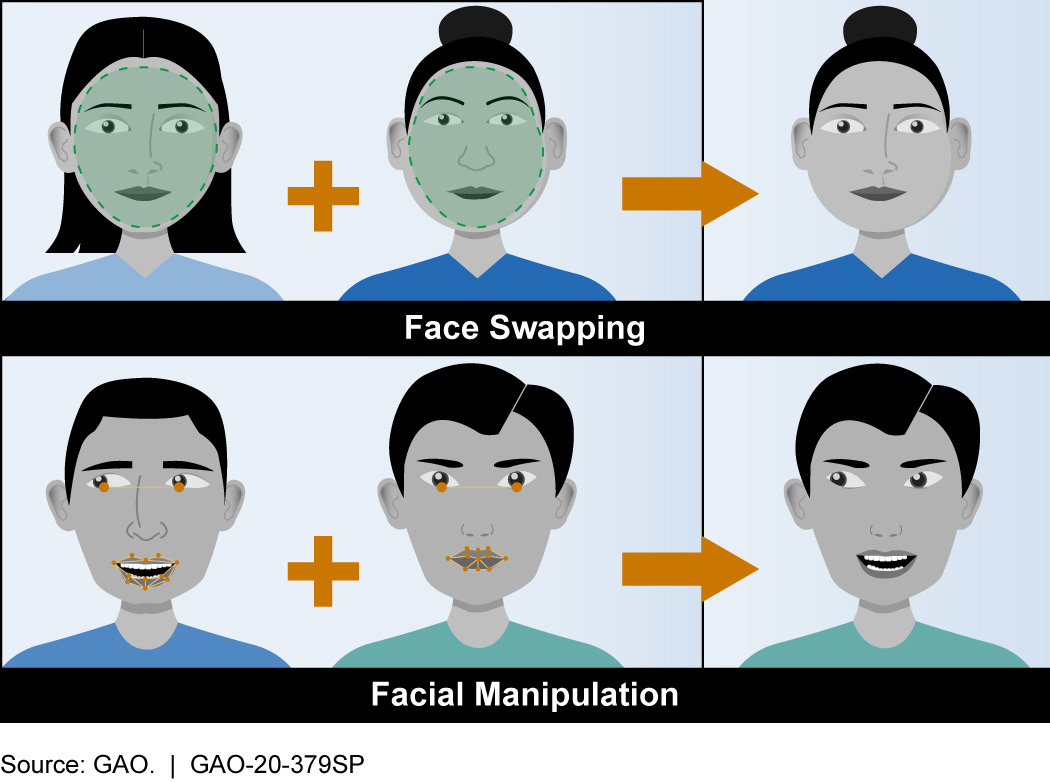
\includegraphics[width=0.9\textwidth]{images/704754.png}  
    \caption{Kasvojen vaihtamisen ja kasvojen manipuloinnin kuvituskuvat (lähde: gao.gov)}  
    \label{figure:deepfakes_fin}  
\end{figure}  

\section*{Puolustuskeinot}

Puolustautuminen tekoälyavusteisia käyttäjän manipulointihyökkäyksiä vastaan on pitkälti samankaltaista kuin perinteisiä, ilman tekoälyn hyödyntämistä toteutettuja manipulointihyökkäyksiäkin vastaan, seuraavilla tärkeillä muutoksilla. Puolustautumiskeinot voidaan karkeasti jakaa tekniikka- ja käyttäjälähtöisiin~\citep{tsinganos_Towards_Automated_Recognition_Chat_SE_Enterprise_2018}.


Perinteinen tapa suojata käyttäjää tietojenkalasteluviesteiltä on esimerkiksi sähköpostiviestien sääntöpohjainen suodattaminen~\citep{mirsky_Threat_Offensive_AI_Organizations_2023}. Yksinkertaistettuna se tarkoittaa joukkoa loogisia sääntöjä, joita seuraamalla voidaan jollakin todennäköisyydellä päätellä, onko viesti tietojenkalasteluviesti vai ei. Sääntöpohjainen suodattaminen ei kuitenkaan toimi hyvin tekoälyavusteista tietojenkalastelua vastaan~\citep{fakhouri_AI_Driven_Solutions_SE_Attacks_2024}.

%koneoppimiseen pohjautuvat
Historiallisesti ei ole ollut tarvetta tarkistaa saatujen kuvien tai videoiden aitoutta, mutta nyt syväväärennösten aikakautena työntekijä ei voi luottaa näkemänsä materiaalin aitouteen, vaan lisävarmistuksia on tehtävä~\citep{mirsky_Creation_Detection_Deepfakes_2021}. Yksi tapa on käyttää tekoälypohjaisia palveluita syväväärennösten tunnistamiseen, samaan tapaan kuin sähköpostiviestitkin tarkistetaan.


Tekoälypohjainen käyttäjän manipulointi tuo joitakin tärkeitä muutoksia käyttäjälähtöisiin puolustuskeinoihin. Ensinnäkään käyttäjät eivät enää voi luottaa siihen, että hyvinkään kirjoitettu viesti ei olisi tietojenkalasteluviesti~\citep{gupta_From_ChatGPT_to_ThreatGPT_2023}. Toiseksi kaikki saatu materiaali, kuten kuvat, äänitiedostot ja videot, saattavat olla syväväärennöksiä, vaikka käyttäjä itse ei huomaisi niissä mitään epätavallista~\citep{blauth_AI_Crime_Overview_Malicious_Use_Abuse_2022}.



Käyttäjälähtöiset tavat ovat käyttäjien kouluttaminen, simuloidut käyttäjän manipulointihyökkäykset, yrityksen tietoturva- ja tietosuojaohjeistusten laatiminen ja käytön valvonta sekä tietoturva- ja tietosuojatietoisen yrityskulttuurin rakentaminen~\citep{tsinganos_Towards_Automated_Recognition_Chat_SE_Enterprise_2018}. Käyttäjille tulee esitellä miltä syväväärennökset näyttävät~\citep{mirsky_Creation_Detection_Deepfakes_2021} sekä kuulostavat~\citep{doan_BTSE_Audio_Deepfake_Detection_2023} ja kuinka helppoa niiden luominen on.



%Koska tekoälyohjelmat pystyvät automaattisesti etsimään Internetistä tietoa, jota voisi käyttää osana käyttäjän manipulointihyökkäyksiä, myöskään viestit, joissa on maininta joistain käyttäjälle oleellista, ehkä jopa henkilökohtaisista asioista, ei voida enää varmuudella sanoa olevan aitoja.

\section*{Johtopäätökset ja suositukset}

Tekoälyavusteisten käyttäjän manipulointihyökkäysten torjuminen pohjautuu siis pitkälti jo käytössä oleviin tekniikoihin: sisääntulevan viestinnän tarkistamiseen, käyttäjien kouluttamiseen, simuloituihin hyökkäyksiin, tietoturva- ja tietosuojatietoisen organisaatiokulttuurin rakentamiseen ja tietoturvasäännösten ylläpitoon sekä niiden käytön toteutumisen valvontaan~\citep{fakhouri_AI_Driven_Solutions_SE_Attacks_2024}. Jokaiseen näihin on kuitenkin tehtävä muutoksia generatiivisen tekoälyn luoman uuden uhan vuoksi, jotta organisaatiot säästyisivät jopa useisiin miljooniin euroihin nousevilta kustannuksilta~\citep{eniza_Threat_Landscape_2024, verizon_Data_Breach_Investigations_Report_2024}.

Tietomurtojen maailmanlaajuisesta tilanteesta tieteellisesti kertovan Cost of a Data Breach Report -raportin~\citep{ibm_Cost_Data_Breach_Report_2024} mukaan käyttäjien koulutukseen panostaminen alensi keskimääräisestä tietoturvahyökkäyksestä koituneita kustannuksia eniten, 258 629 dollarilla. Vertailun vuoksi tietoturvaohjelmistoihin panostamalla keskimääräiset kustannukset olivat 166 600 dollaria pienemmät. Organisaatioiden jotka panostivat vain vähän käyttäjien tietoturvakoulutukseen keskimääräiset tietomurroista aiheutuneet kustannukset vuositasolla olivat \$5,1 miljoonaa, kun vastaava luku hyvin koulutettujen käyttäjien organisaatioilla oli \$4,15 miljoonaa.



Voimme siis olettaa tekoälyjärjestelmien nopean kehittymisen jatkuvan, tietoturvauhkien kehittymisen niiden mukana sekä tarpeen jatkuvaan käyttäjien kouluttamiseen ja uusien puolustuskeinojen löytämiseen kasvavan. Organisaatioiden tulee huomioida generatiivisen tekoälyn käyttäjän manipulointihyökkäyksiin mukanaan tuomat uudet erityispiirteet panostamalla ensisijaisesti työntekijöidensä koulutukseen ja toissijaisesti uusiin tekoälypohjaisiin tietoturvaohjelmistoihin.





\end{otherlanguage}


